\section{Latency}\label{app_sec:latency}
Here's a concise table comparing the latency of pure decoding to the additional delay introduced by grammar constraints.


\xhdr{Latency for IE}
We provide a measurement of latency for IE task in Figure~\ref{fig:latency_wikiner} and Figure~\ref{fig:latency_rebel}.
We consider two large grammars, the WikiNER grammar and the REBEL grammar.
The WikiNER grammar contains 279 K entities and 158 relations.
The REBEL grammar contains 5.9 M entities and 857 relations.
%
Given the grammar, we randomly pick the next token from the set of next allowed tokens with the end-of-sentence token excluded to avoid early termination.
%
The incremental parsing step is done on CPU and we do not use any optimization techniques such as multi-threading.

\begin{figure}[ht]
  \centering
  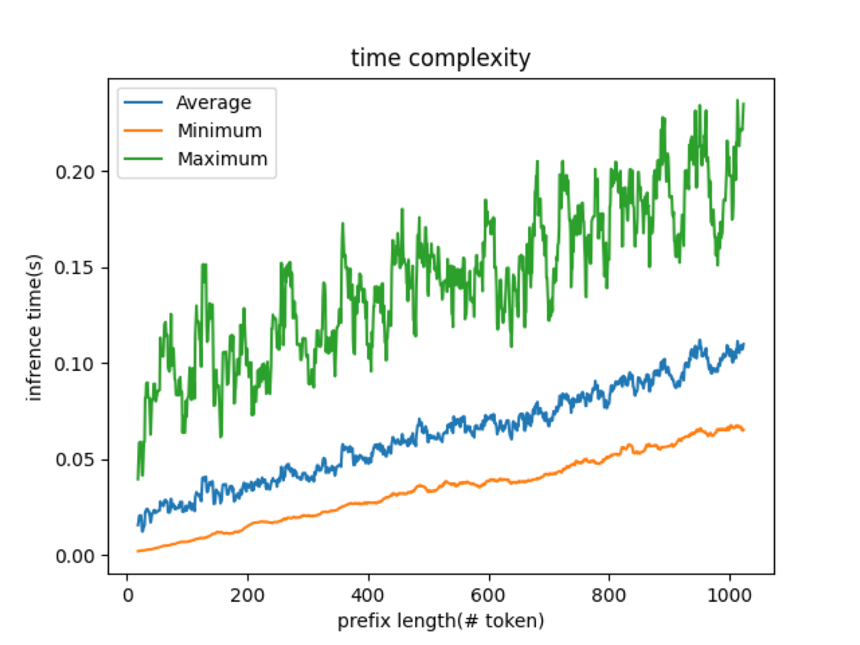
\includegraphics[width=0.45\textwidth]{img/latency/wiki_ner}
  \caption{latency of WikiNER grammar}
  \label{fig:latency_wikiner}
\end{figure}

\begin{figure}[ht]
  \centering
  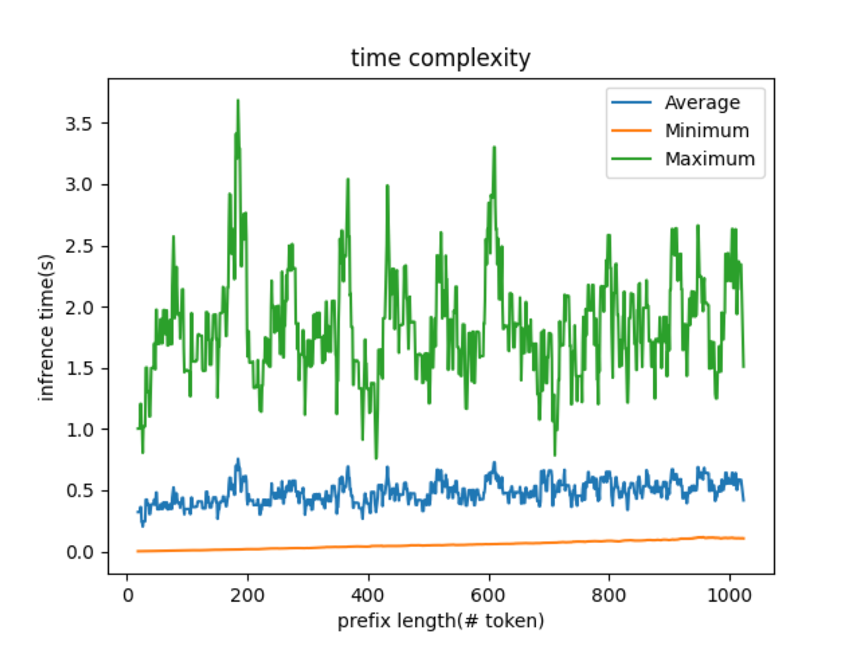
\includegraphics[width=0.45\textwidth]{img/latency/rebel}
  \caption{latency of REBEL grammar}
  \label{fig:latency_rebel}
\end{figure}



As shown in Figure~\ref{fig:latency_wikiner}s, the latency for WikiNER grammar (0.05s) is comparable to the latency of the LM on GPU.
However, the latency for the REBEL grammar (0.5s) is significantly higher than the latency of the LM.
We believe this can be largely improved by using more appropriate incremental parser and leave it as future work.




